\chapter{Two-player Yorke's game of survival in chaotic transients} %7P5
\label{chap:PartialControlGame}


\begin{quotation}

	\vspace{-3cm}
	\begin{flushright}
    \begin{minipage}[t][5cm][b]{0.5\textwidth}
    {\letquote ``As a general rule, the most successful man in life is the man who has the best information.''}
    
    \bigskip
    
    -{\small  Benjamin Disraeli}
    \end{minipage}
    \end{flushright}



    \vspace{0.5cm}

\end{quotation}




In the previous chapter we developed a method of partial control that followed the line of work initiated in \cite{Yorke} followed by papers on the issue \cite{DynamicsPartialControl,PartialControlBeyond,PartialControlFunctions} among others. The study led to the publication of \cite{PartialControlEscape}. 

The problem introduced in \cite{Yorke} was devised as a kind of game where one player is at a huge disadvantage but, nonetheless, can achieve its goal. From there on the studies derived in a control method that did not force a single trajectory as the solution, but provided a set of points, the \textit{safe sets}, where the controller was safe; hence the name \textit{partial control}.

On the other hand, game theory provides powerful tools for analyzing strategic interactions across diverse fields, from social sciences to economics and physics \cite{Social,EconomyGames,GamesComplex}. While classical game theory typically focuses on equilibrium states, many real-world situations involve chaotic systems, where extreme sensitivity to initial conditions and inherent unpredictability create fundamental challenges for strategic decision-making. The nonlinear nature of these systems makes traditional game-theoretic approaches insufficient, as small perturbations can lead to dramatically different outcomes. What's more, the intrinsic characteristics of a game are susceptible to change in real life, and these changes can result from the players' decisions \cite{AkiyamaKaneko1,AkiyamaKaneko2}.

Game theory has also proven valuable in chaos control \cite{GamesControl}, where control problems naturally emerge as competitive scenarios between opposing objectives. This framework reveals how controllers must optimize their strategies while dealing with three key challenges: (1) the unpredictable nature of chaotic dynamics, (2) the system constraints, and (3) the actions of other controllers who must carefully choose their actions to achieve their own goal. This interaction between different control agents adds a strategic dimension that goes beyond traditional chaos control methods.

Since this thesis is oriented towards game dynamics, the opportunity to rejoin this two branches of the problem led to the publication of \cite{PartialControlGame}. In this paper we present a two-player game of control where each player has conflicting objectives. One player wants to control the trajectory of a given dynamical system towards one region and the opponent towards a different one. Through the analysis of the game with the partial control tools we achieve the solution of the game through all initial conditions. We will construct the \textit{winning sets} (what was previously called \textit{safe sets}), as the initial conditions that guarantee victory for each player.

To illustrate the game we studied a paradigmatic dynamical system, the logistic map ${f(x) = \mu x_n(1-x_n)}$. The system presents transient chaotic dynamics for $\mu>4$ where all orbits starting at the region $Q=[0,1]$ eventually leave the region in a finite time. When one player aims to stay at the region $Q$ indefinitely and the other aims to drive the trajectory off, the game gets very interesting. In one hand, the game is asymmetric since the player who wants to leave region $Q$ is in advantage. On the other hand, we found that there are initial conditions where the player that aims to conserve the trajectory in the transient region can do so even when their control is lesser than the opponent's control.

In many games the order of play is important. This game is no exception, here the importance lies in the information that the second player has when they see the action of the opponent. Knowing where the opponent is going to push the trajectory to will affect the decision of control of the second player, giving them an advantage that the first player lacks. To study this effect, we devised three scenarios. In the first game the player that aims to keep the trajectory in the region $Q$ knows the action of the rival. In the second one, the informed player is the one who intends to expel the trajectory form the region. Finally, in the third game, no player knows the rival's action. The lack of knowledge in this last game will translate in the unsettled solution of the game. Regions where no player has the victory assured appear as a consequence of these lack of knowledge.


\section{The game}


\begin{figure}
    \centering
    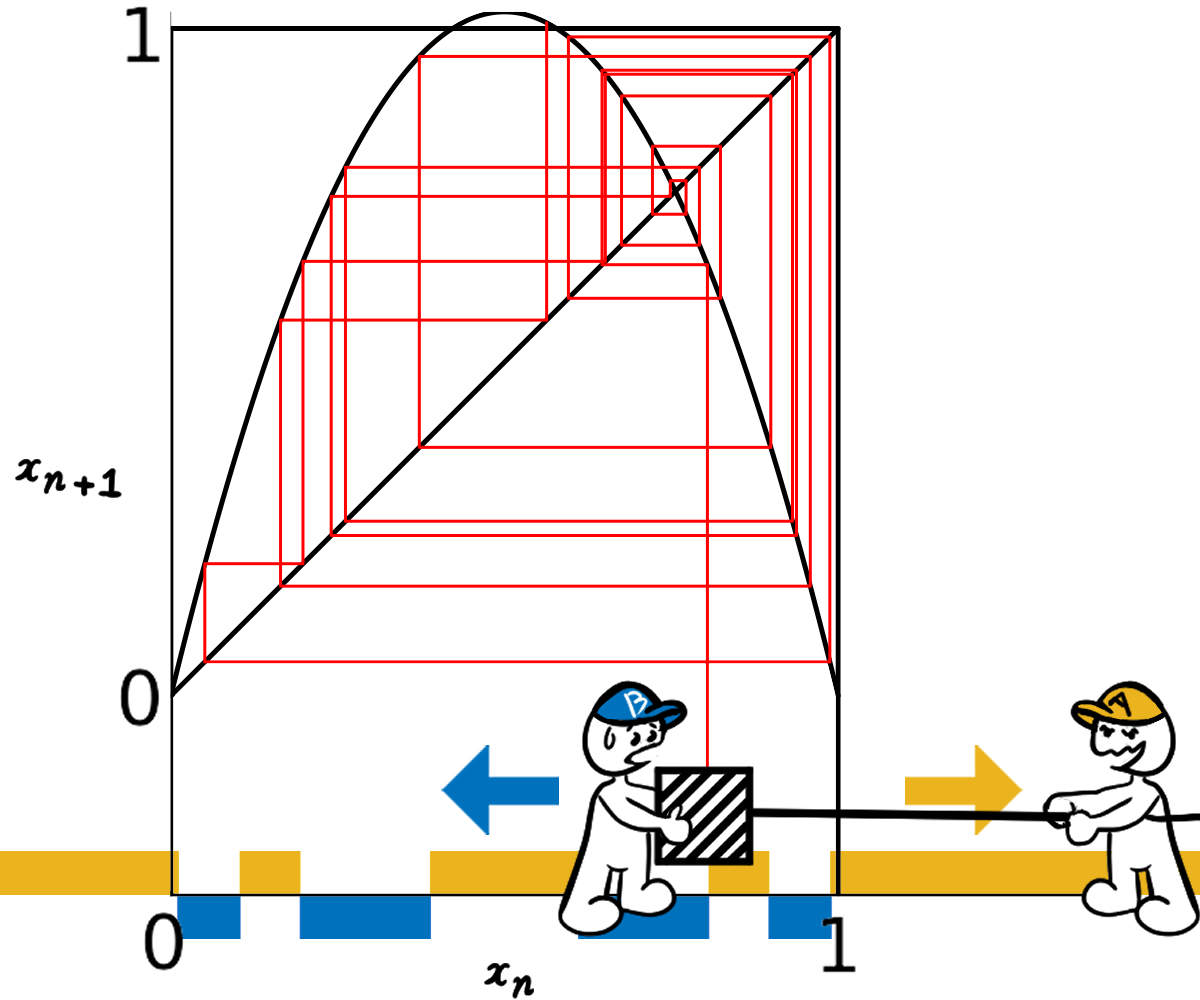
\includegraphics[width=0.7\textwidth]{Images/P5/drawing.png}
    \caption{Players $A$ and $B$ compete for controlling the trajectory on the chaotic and escaping logistic map $x_{n+1} = \mu x_n(1-x_n)$. Player $B$ tries to maintain the trajectory on the region $Q = [0,1]$, while fighting against the dynamics of the map, since for $\mu > 4$ all points except a zero measure Cantor set eventually escape from the region. The red line shows an example of one orbit that ends up escaping. Furthermore, player $B$ also fights against the opponent, player $A$, who aims to expel the trajectory from region $Q$ in a finite time. To achieve their goals the players can control the trajectory with a given control bound. The yellow and blue rectangles are the \textit{winning sets} of players $A$ and $B$, respectively. These are the initial conditions that guarantee victory for each player.}
    \label{fig:drawing}
\end{figure}



Consider two individuals pulling an object. Player A aims to pull the object to their side, while Player B pulls it toward their own. In the absence of any other factors, the stronger player will prevail by exerting more force. However, the game becomes much more interesting when the movement of the object is influenced by a natural dynamic governed by a rule defined by a function $f$. In this case, the players must not only consider their opponent's force but also account for the inherent motion of the object. This becomes more challenging when the movement that describes $f$ is chaotic. In such scenarios, even slight variations in how the players pull can result in entirely different and unpredictable outcomes, as illustrated in Fig.~\ref{fig:drawing}.  



With this in consideration, we formulate our game. Let $Q$ represent a region in the phase space, with a map $f$ acting on the state space $X$. The initial state $x$ of the game begins within $Q$. Player $B$'s objective is to keep the trajectory within $Q$, while player $A$'s goal is to drive the trajectory outside of $Q$. Each iteration of the game involves players $A$ and $B$ selecting their respective bounded controls, $u_n^A$ and $u_n^B$. At each discrete time step $n$, the state $x_n$ evolves according to this dynamics
\begin{equation}
    x_{n+1} = f(x_n) + u_n^A + u_n^B,
\end{equation}
where $u_n^A $ and $u_n^B $ represent the control actions of players $A$ and $B$, respectively. These controls are bounded by
\begin{equation}
    |u_n^A| \leq u_0^A, \quad |u_n^B| \leq u_0^B.
\end{equation}


Player $B$ wins if the trajectory remains inside $Q$ indefinitely, whereas player $A$ wins if the trajectory exits $Q$. Once the trajectory has left $Q$, player $B$ has no chance of returning it to the region.

A crucial factor in solving this game is the order of play. To address this, we consider three distinct scenarios summarized in Table~\ref{tab:games}. In game $A^{-}B^{+}$, player B has the advantage of knowing the actions of player $A$ before making their move. This sequential structure allows player $B$ to respond optimally to the choices of their rival. In game $A^{+}B^{-}$, player $A$ has the advantage, with complete knowledge of moves by player $B$ before acting. Finally, in game $A^{-}B^{-}$, both players make their decisions simultaneously, without any knowledge of the opponent actions.  



\begin{table}[h!]
\centering
\begin{tabular}{|p{3cm}|p{4cm}|p{7.3cm}|}
\hline
\textbf{Game Type} & \textbf{Order of Play} & \textbf{Information Available} \\
\hline
Game $A^{-}B^{+}$ & $B$ plays after $A$ & B knows $A$'s action  \\
\hline
Game $A^{+}B^{-}$ & $A$ plays after $B$ & $A$ knows $B$'s action  \\
\hline
Game $A^{-}B^{-}$ & Simultaneous play & Both ignore the opponent's action  \\
\hline
\end{tabular}
\caption{Three different scenarios analyzed in this paper based on the order of play, i.e., what information is available to each player.}
\label{tab:games}
\end{table}











\section{Solving the game: The winning sets}




\begin{figure}[h!]
    \centering
    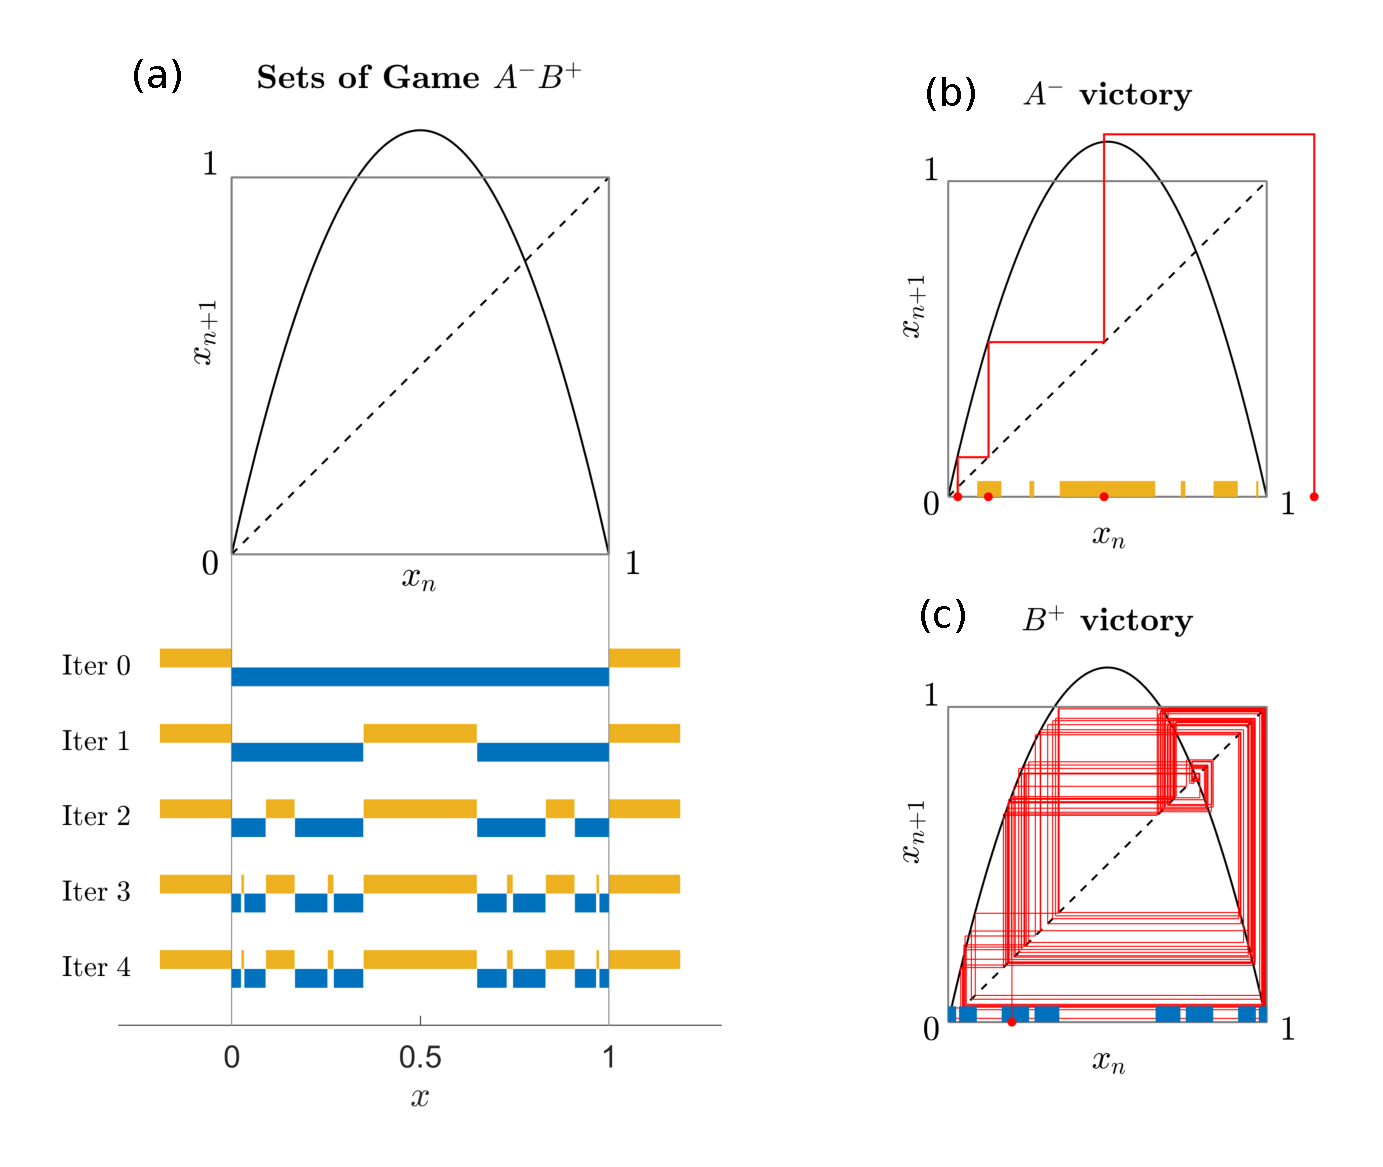
\includegraphics[trim={0.8cm 0cm 0cm 0cm}, clip,width=0.95\textwidth ]{Images/P5/setsAB_control.eps}
    \caption{ Winning sets and controlled trajectory for a game between an ignorant player $A$ and an informed player $B$. (a) Steps of the algorithm to compute the winning sets for the ignorant player $A$, $W^{A^-}$, in yellow, and for the informed player $B$, $W^{B^+}$, in blue. The sets were computed in the region $R\in [-0.3,1.3]$, with $Q\in[0,1]$, $u_0^A=0.016$, $u_0^B=0.038$. The algorithm converges in $3$ iterations since  the sets for the third iteration are identical to those of the forth. (b) Controlled trajectory of the game when the initial condition belongs to player's $A$ winning set. Player $A$ acts first, without knowledge of player $B$'s move, so they choose its control at each step to reach the closest point belonging to the shrunk set ($W^{A^-} -u^B_0$), accounting for the worst possible subsequent action of player $B$. After $3$ iterations the trajectory has left region $Q$, so player $A$ wins. (c) The game now starts in a point that belongs to player's $B$ winning set. Player $B$ acts second, with the knowledge of player $A$'s move, so selects their control to reach the closest point belonging to set $W^{B^+}$. The trajectory stays indefinitely inside region $Q$, so player $B$ wins as long as control is maintained.}
    \label{fig:tray}
\end{figure}



\begin{figure}[h!]
    \centering
   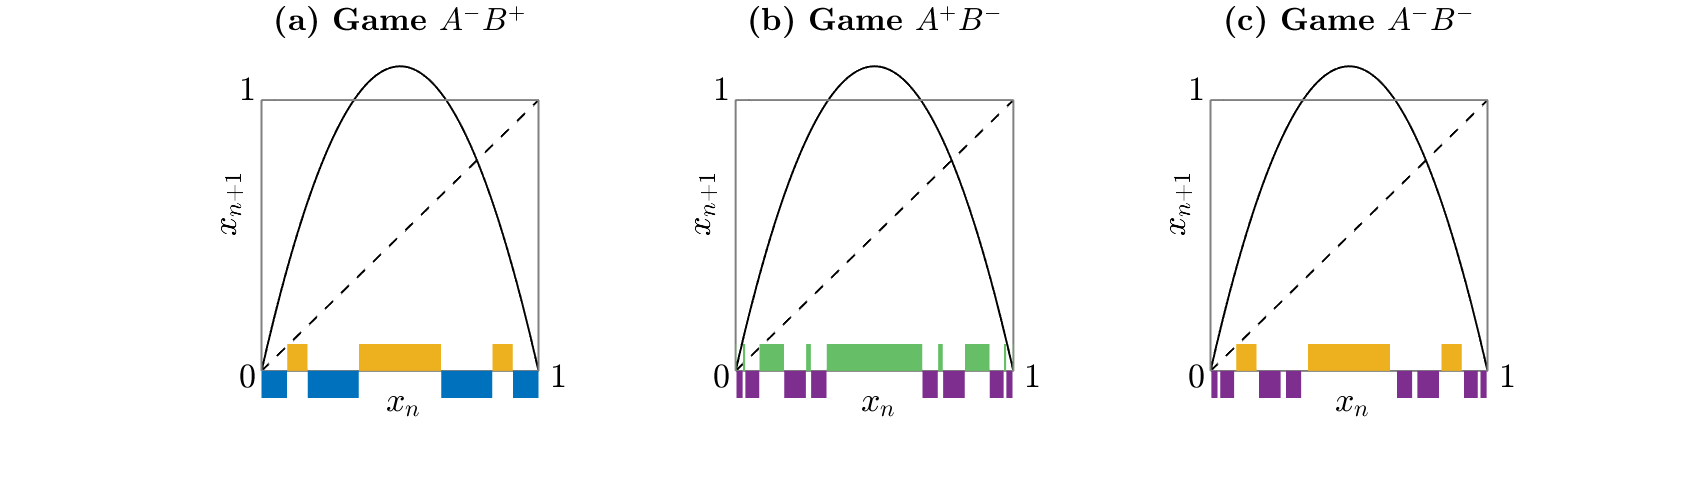
\includegraphics[trim={3.2cm 0cm 0cm 0cm}, clip,width=1.1\textwidth ]{Images/P5/sets_juego.png}
    \caption{The logistic map and winning sets to control trajectories of the logistic map with $\mu = 4.5$ and control bounds $u^A_0 = 0.015$ for player $A$, and $u^B_0 = 0.040$ for player $B$. Each winning set at the bottom show the initial conditions that guarantee victory to each player. Each player has two winning sets whether they are informed ($+$) or ignorant ($-$) to their opponent's move. The winning sets of player $A$ are colored in green when they are informed and in yellow when they are ignorant. On the other hand, those of player $B$ are colored in blue when they are informed and purple when they are ignorant. For simplicity, we only represent the winning sets in the interval $Q$. (a) Ignorant player $A$ against informed player $B$ (b) Now the informed player is $A$ who plays against the ignorant player $B$ (c) Neither player knows each other actions. In this case, there are regions that do not belong to any player's winning set, meaning that both player could win when starting at those initial conditions, but the victory is uncertain because players cannot guarantee victory against any move from the opponent. These "no winning regions" represent the difference between the respective informed winning sets and the ignorant winning sets.}
    \label{fig::sets}
\end{figure}




Given the opposing objectives described in the previous section, we define a region $R$, containing $Q$, where the winning sets $W$ are determined for both players. These sets represent whether a given initial condition guarantees victory (value $1$) or not (value $0$). For Player $B$, the initial condition is $W^B(x) = 1$ for $x \in Q$ and $0$ otherwise. Conversely, for Player $A$, the initial condition is $W^A(x) = 0$ for $x \in Q$ and $1$ otherwise.  

The computation process for each winning set depends on whether the player is informed by knowing the opponent's move, or ignorant. This procedure is summarized in Table~\ref{tab:morphological_operations}. Each set can be computed independently, as outlined below:  

\begin{itemize}
\item {\bf Player $A^-$ (ignorant player $A$):}
To compute the set of $W^{A^-}$, we have to evaluate for each $x \in Q$ the image $f(x)+u^A+u_0^B$ for all possible controls $u^A \in [-u_0^A,u_0^A]$ and $u^B \in [-u_0^B,u_0^B]$. We select only those $u^A$ where all possible images $f(x)+u^A+[-u_0^B,u_0^B]$ fall within $W^{A^-}$. Points $x \in Q$ satisfying this condition update $W^{A^-}(x)=1$. All these initial conditions are able to be controlled to escape after one iteration of the map. But there will be other points that, after more than one iterations of the map and control, will be able to escape. To find this points we must repeat the algorithm, thus updating $W^{A^-}$ until it converges.

This process is equivalent to performing the following morphological operations: first shrinking $W^{A^-}$ by $u_0^B$, then dilating by $u_0^A$. For any $x \in Q$ whose $f(x)$ falls within the shrunk set, we set $W^{A^-}(x)=1$. The process is repeated with this new $W^{A^-}$ until it converges.

\item {\bf Player $A^+$ (informed player $A$):}
To compute the set of $W^{A^+}$, we analyze $f(x)+u^B+u^A$ for all possible controls. For each $x \in Q$, we evaluate $f(x)+[-u_0^B,u_0^B]+u^A$ and determine if there exists some $u^A \in [-u_0^A,u_0^A]$ capable of forcing escape for all possible images. If such $u^A$ exists, then $W^{A^+}(x)=1$. This process is performed for all $x \in Q$, updating the set $W^{A^+}$. The algorithm is repeated until $W^{A^+}$ converges.

Morphologically, this process is equivalent to first dilating $W^{A^+}$ with $u_0^A$ and then shrinking the resulting set with $u_0^B$. For any $x \in Q$ whose $f(x)$ falls within this shrunk set, we set $W^{A^+}(x)=1$.

\item {\bf Player $B^-$ (ignorant player $B$):}
To compute the set of $W^{B^-}$, we evaluate for each $x \in Q$ the image $f(x)+u^B+u_0^A$ for all possible controls $u^B \in [-u_0^B,u_0^B]$ and $u^A \in [-u_0^A,u_0^A]$. We select only those $u^B$ where all possible images $f(x)+u^B+[-u_0^A,u_0^A]$ fall within $W^{B^-}$. Points $x \in Q$ not satisfying this condition update $W^{B^-}(x)=0$. Since player $B$ wants to keep the orbit in $Q$ forever, the algorithm must be repeated until $W^{B^-}$ converges.

The process is equivalent to iteratively performing the following morphological operations: first shrinking $W^{B^-}$ by $u_0^A$, then dilating by $u_0^B$. For any $x \in Q$ whose $f(x)$ falls outside the shrunk set, we set $W^{B^-}(x)=0$. The process is repeated with this new $W^{B^-}$ until it converges.

\item {\bf Player $B^+$ (informed player $B$):}
To compute the set of $W^{B^+}$, we analyze $f(x)+u^A+u^B$ for all possible controls. For each $x \in Q$, we evaluate $f(x)+[-u_0^A,u_0^A]+u^B$ and determine if there exists some $u^B \in [-u_0^B,u_0^B]$ capable of guaranteeing containment for all possible images. If such $u^B$ does not exist, then $W^{B^+}(x)=0$. This process is performed for all $x \in Q$, updating the set $W^{B^+}$. The algorithm is repeated until $W^{B^+}$ converges.

Morphologically, this process is equivalent to first dilating $W^{B^+}$ with $u_0^B$ and then shrinking the resulting set with $u_0^A$. For any $x \in Q$ whose $f(x)$ falls outside this shrunk set, we set $W^{B^+}(x)=0$.
\end{itemize}




\begin{table}[h]
\centering
\begin{tabular}{|c|c|>{\raggedright\arraybackslash}p{9.5cm}|}
\hline
Player & Initial Set & \multicolumn{1}{c|}{Morphological Operations} \\
\hline
$A^-$ & 
$\begin{array}{l} 
W^{A^-}(x)=\begin{cases} 
0 & x \in Q \\
1 & \text{otherwise}
\end{cases} \\
\\
W^{A^-}_{\text{new}}=W^{A^-}
\end{array}$ 
& $\begin{array}{l} \\ 
1. \text{ Shrink } W^{A^-} \text{ by } u_0^B \text{ to obtain } W^{A^-}_{\text{shrunk}} \\ 2. \text{ Dilate } W^{A^-}_{\text{shrunk}} \text{ by } u_0^A \text{ to obtain } W^{A^-}_{\text{dilated}} \\ 3. \text{~} \forall x \in Q, \text{ if } f(x) \text{ falls in } W^{A^-}_{\text{dilated}},\text{ set }W^{A^-}_{\text{new}}(x)=1 \\  4. \text{~} W^{A^-}=W^{A^-}_{\text{new}}. \text{ Go to step 1 and repeat the process} \\ ~
\end{array}$ \\ \hline
$A^+$ & $\begin{array}{l}
W^{A^+}(x)=\begin{cases}
0 & x \in Q \\
1 & \text{otherwise}
\end{cases} \\
\\
W^{A^+}_{\text{new}}=W^{A^+}
\end{array}$ 
& $\begin{array}{l} \\ 
1. \text{ Dilate } W^{A^+} \text{ by } u_0^A \text{ to obtain } W^{A^+}_{\text{dilated}} \\ 2. \text{ Shrink } W^{A^+}_{\text{dilated}} \text{ by } u_0^B \text{ to obtain } W^{A^+}_{\text{shrunk}} \\ 3. \text{~} \forall x \in Q, \text{ if } f(x) \text{ falls in } W^{A^+}_{\text{shrunk}},\text{ set }W^{A^+}_{\text{new}}(x)=1 \\  4. \text{~} W^{A^+}=W^{A^+}_{\text{new}}. \text{ Go to step 1 and repeat the process} \\ ~
\end{array}$ \\ \hline
$B^-$ & $\begin{array}{l}
W^{B^-}(x)=\begin{cases}
1 & x \in Q \\
0 & \text{otherwise}
\end{cases} \\
\\
W^{B^-}_{\text{new}}=W^{B^-}
\end{array}$ 
& $\begin{array}{l} \\ 
1. \text{ Shrink } W^{B^-} \text{ by } u_0^A \text{ to obtain } W^{B^-}_{\text{shrunk}} \\ 2. \text{ Dilate } W^{B^-}_{\text{shrunk}} \text{ by } u_0^B \text{ to obtain } W^{B^-}_{\text{dilated}} \\ 3. \text{~} \forall x \in Q, \text{ if } f(x) \text{ falls in } W^{B^-}_{\text{dilated}},\text{ set }W^{B^-}_{\text{new}}(x)=1 \\  4. \text{~} W^{B^-}=W^{B^-}_{\text{new}}. \text{ Go to step 1 and repeat the process} \\ ~
\end{array}$ \\ \hline
$B^+$ & $\begin{array}{l}
W^{B^+}(x)=\begin{cases}
1 & x \in Q \\
0 & \text{otherwise}
\end{cases} \\
\\
W^{B^+}_{\text{new}}=W^{B^+}
\end{array}$ 
& $\begin{array}{l} \\ 
1. \text{ Dilate } W^{B^+} \text{ by } u_0^B \text{ to obtain } W^{B^+}_{\text{dilated}} \\ 2. \text{ Shrink } W^{A^+}_{\text{dilated}} \text{ by } u_0^A \text{ to obtain } W^{B^+}_{\text{shrunk}} \\ 3. \text{~} \forall x \in Q, \text{ if } f(x) \text{ falls in } W^{B^+}_{\text{shrunk}},\text{ set }W^{B^+}_{\text{new}}(x)=1 \\  4. \text{~} W^{B^+}=W^{B^+}_{\text{new}}. \text{ Go to step 1 and repeat the process} \\ ~
\end{array}$ \\ \hline
\end{tabular}
\caption{Morphological operations for each player's winning set computation.}
\label{tab:morphological_operations}
\end{table}



%TODO Rewrite



\section{Game of survival in the logistic map}

To demonstrate our method, we explore a game based on the logistic map, \linebreak ${f(x) = \mu x_n(1-x_n)}$ with $\mu=4.5$ and $Q=[0,1]$. This map provides an ideal scenario due to its transient chaotic behavior within $Q$: the trajectories exhibit chaotic dynamics before eventually leaving the region. This creates an asymmetric situation where Player $B$, aiming to keep the trajectory inside the region, must contend with both the natural behavior of the system and the opposing player’s objective of pushing the trajectory out. While this example is specific, our approach can be generalized to other maps $f$ and regions $Q$ in the phase space.

In this setup, both players are allowed to apply control at each step to influence the trajectory. However, the control actions of both players are constrained by their respective limits, $u_0^A$ and $u_0^B$. The state of the system after each iteration is given by
\begin{equation}
x_{k+1} = f(x_k) + u^A + u^B,
\end{equation}
where $u^A$ and $u^B$ denote the control that the players exert.

We present a specific example of the game with control bounds $u_0^A = 0.016$ and $u_0^B = 0.038$. In Fig.~\ref{fig:tray}, we illustrate how the winning sets are formed. As the process progresses, the winning sets evolve with each iteration: player $A$’s set grows, while player $B$’s set shrinks. Additionally, two controlled trajectories are shown. The first one, in Fig.~\ref{fig:tray}(b), starting in player $A$’s winning set, where the controller successfully pushes the trajectory out of region $Q$. For the second one, in Fig.~\ref{fig:tray}(c), the trajectory starts in player $B$’s winning set, so they can keep the trajectory within the region.

Figure~\ref{fig::sets} displays the outcomes of three different examples of games, depending on whether each player has knowledge of the other’s actions. In Fig.~\ref{fig::sets}(a), player $A$ moves first, followed by player $B$, therefore player $A$ has advantage by knowing player $B$'s actions. Figure~\ref{fig::sets}(b) reverses the order, with Player $B$ moving first and Player $A$ second. Finally, Fig.~\ref{fig::sets}(c) shows the case where both players are unaware of each other’s moves, representing a simultaneous play situation.

This last game is noteworthy. In this case, regions in the state space appear that do not belong to any winning set. These areas arise because neither player can secure a win without considering the opponent’s strategy. This uncertainty stems from the fact that each player is unaware of the other’s choice when making their decision. As a result, the outcome depends on the specific combination of moves made by both players, and the players may not always respond optimally to the opponent's move.

This uncertainty stands in contrast to the games in Fig.~\ref{fig::sets}(a) and (b), where the presence of informed players leads to clear winning sets, leaving little ambiguity about the game’s outcome for all initial conditions.



\subsection{Exploring possible games in the $(u_0^B,u_0^A)$ space}

\begin{figure}
    \centering
    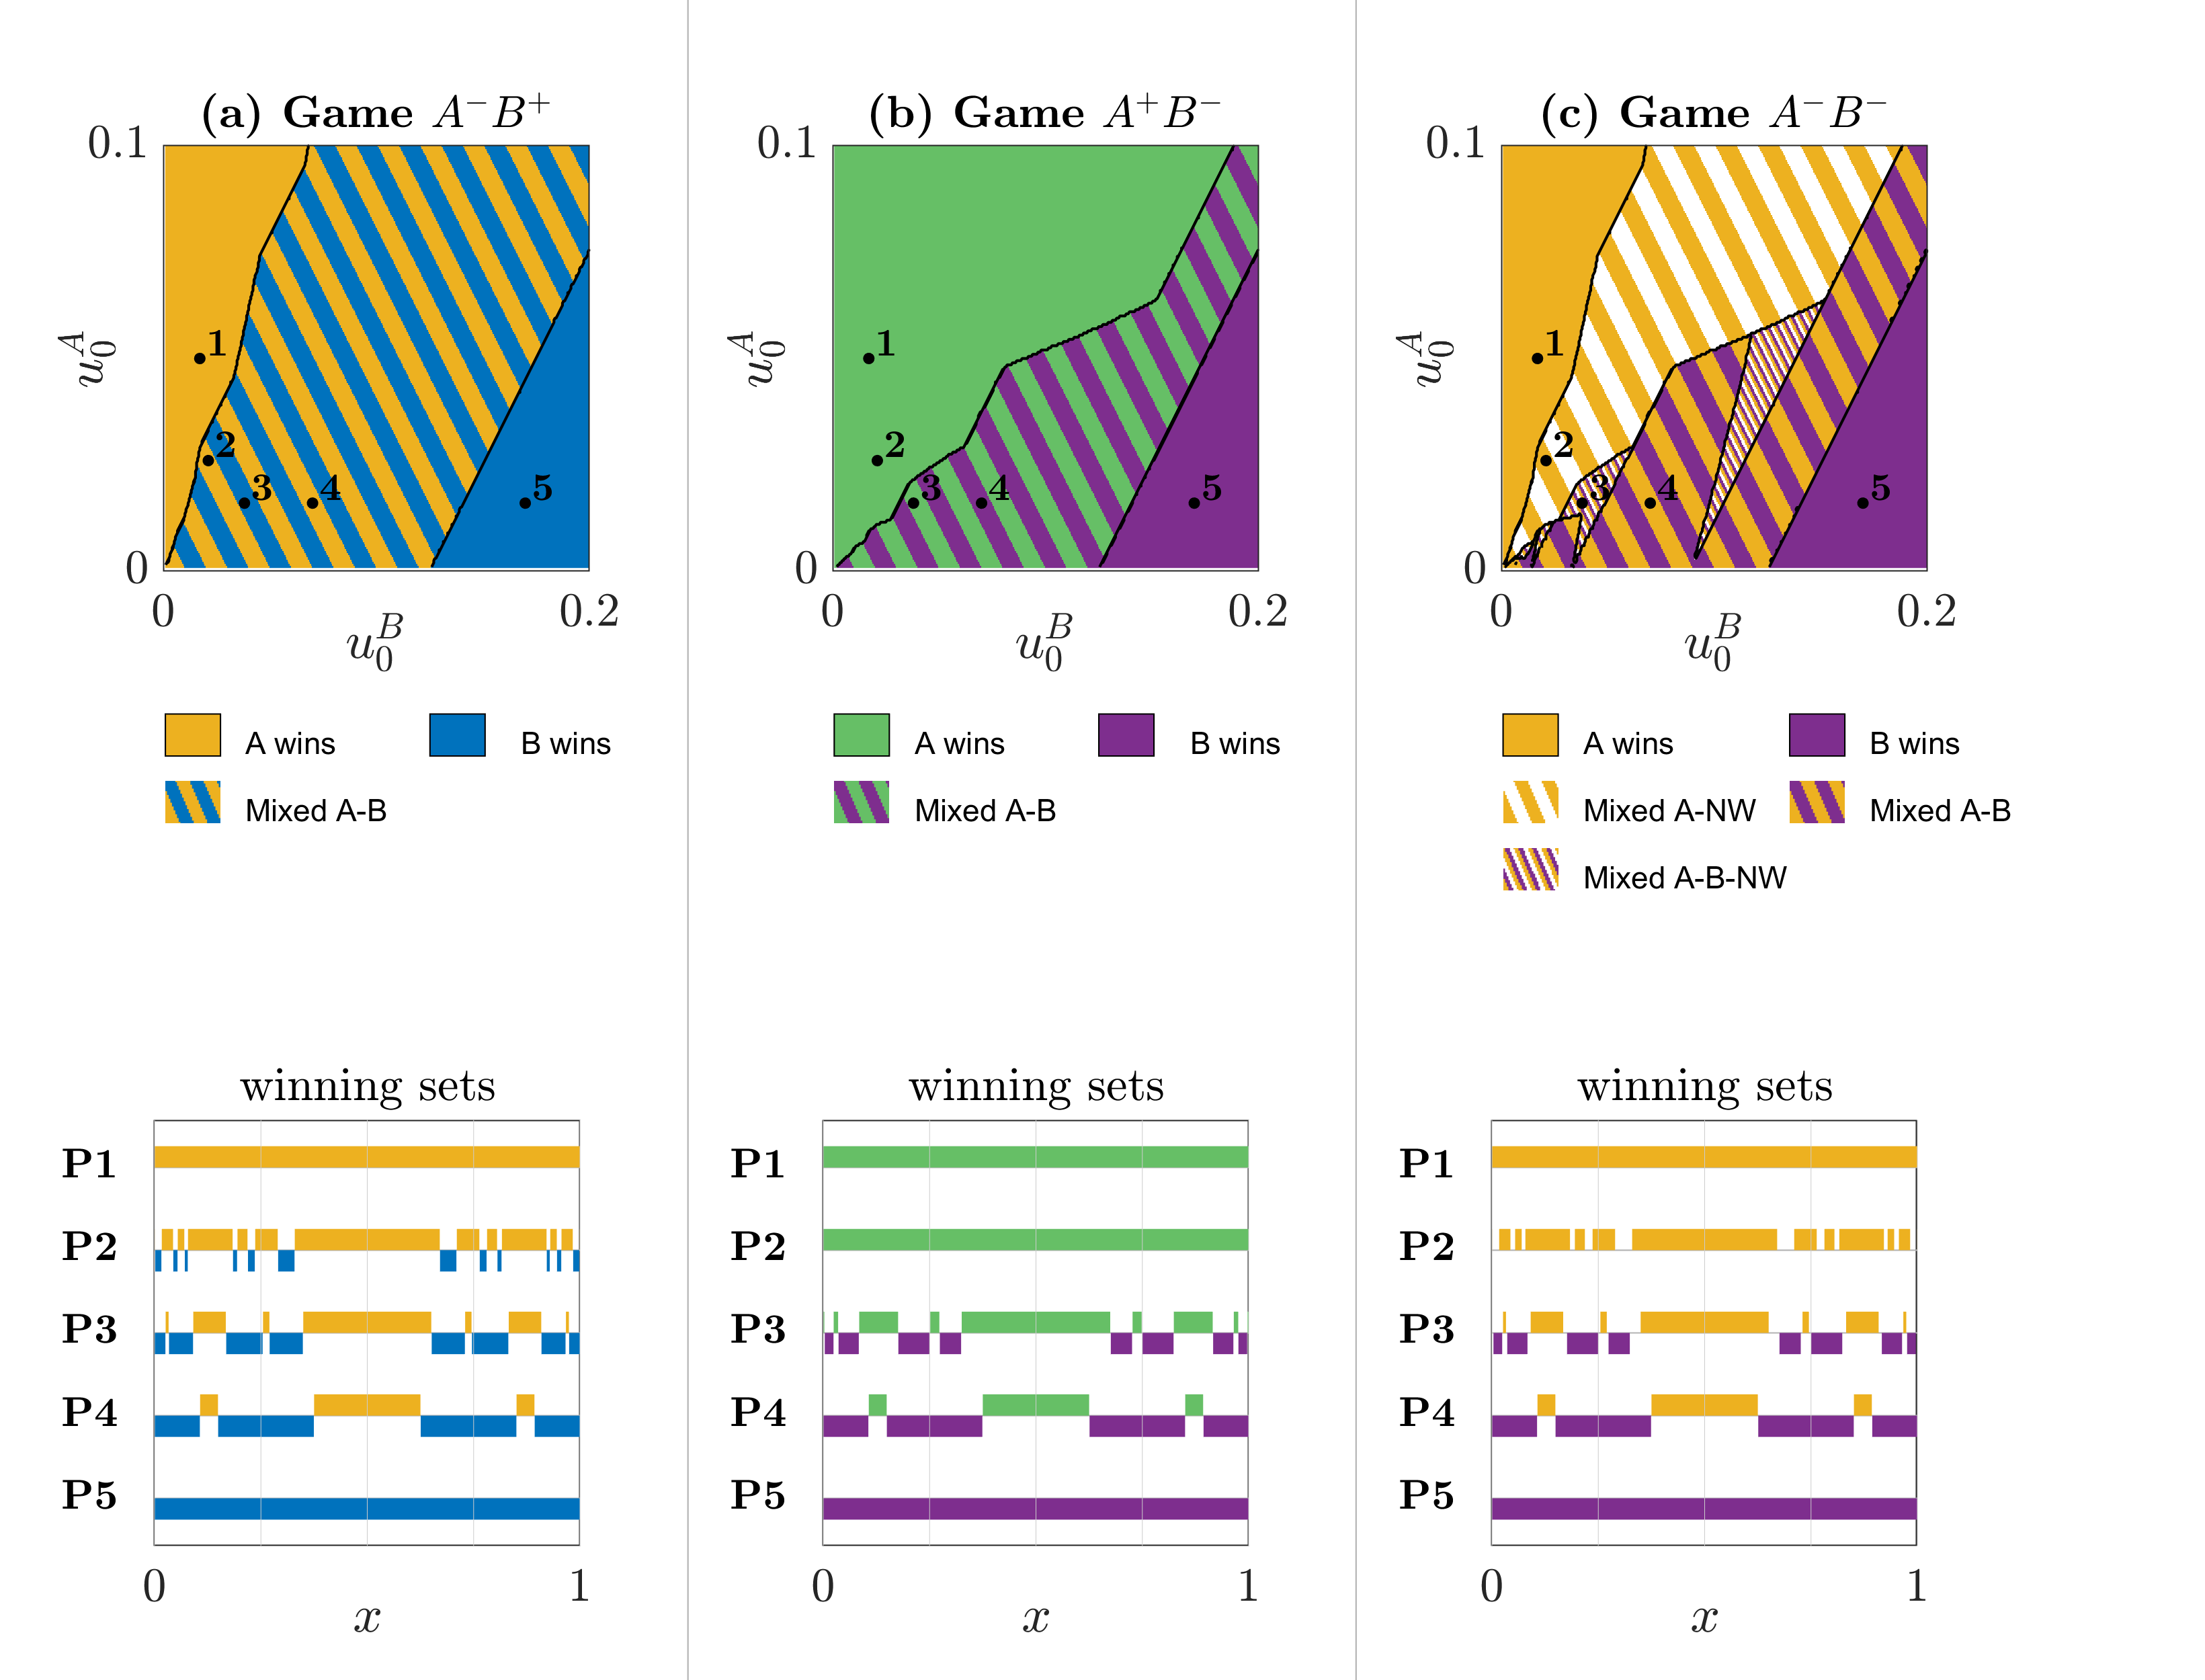
\includegraphics[trim={0.6cm 0cm 0cm 0cm}, clip,width=1.12\textwidth ]{Images/P5/franjas5.png}
    \caption{Different solutions depending on the values of $u^A_0$ and $u^B_0$. Panels (a), (b), and (c) show a diagram in which solid colored regions represent parameter combinations where the informed/ignorant player $A$ wins for all initial conditions at solid colors green/yellow and the informed/ignorant player $B$ at solid blue/purple. Striped regions indicate parameters where the winner depends on the initial conditions. There are also regions with white strips marked as $NW$ (no winning), where the victory is uncertain at some initial conditions. Below each diagram we show the winning sets, i.e., the initial conditions that guarantee victory for each players, for each kind of game at $5$ different regions of control bound. These points, written as $(u^B_0, u^A_0)$, are: $P1 =  (0.017, 0.050)$, $P2 =  (0.021, 0.026)$, $P3 =  (0.038, 0.016)$, $P4=  (0.070, 0.016)$, and $P5= (0.170, 0.016)$. 
    }
    \label{fig:franjas}
\end{figure}


\begin{figure}
    \centering
    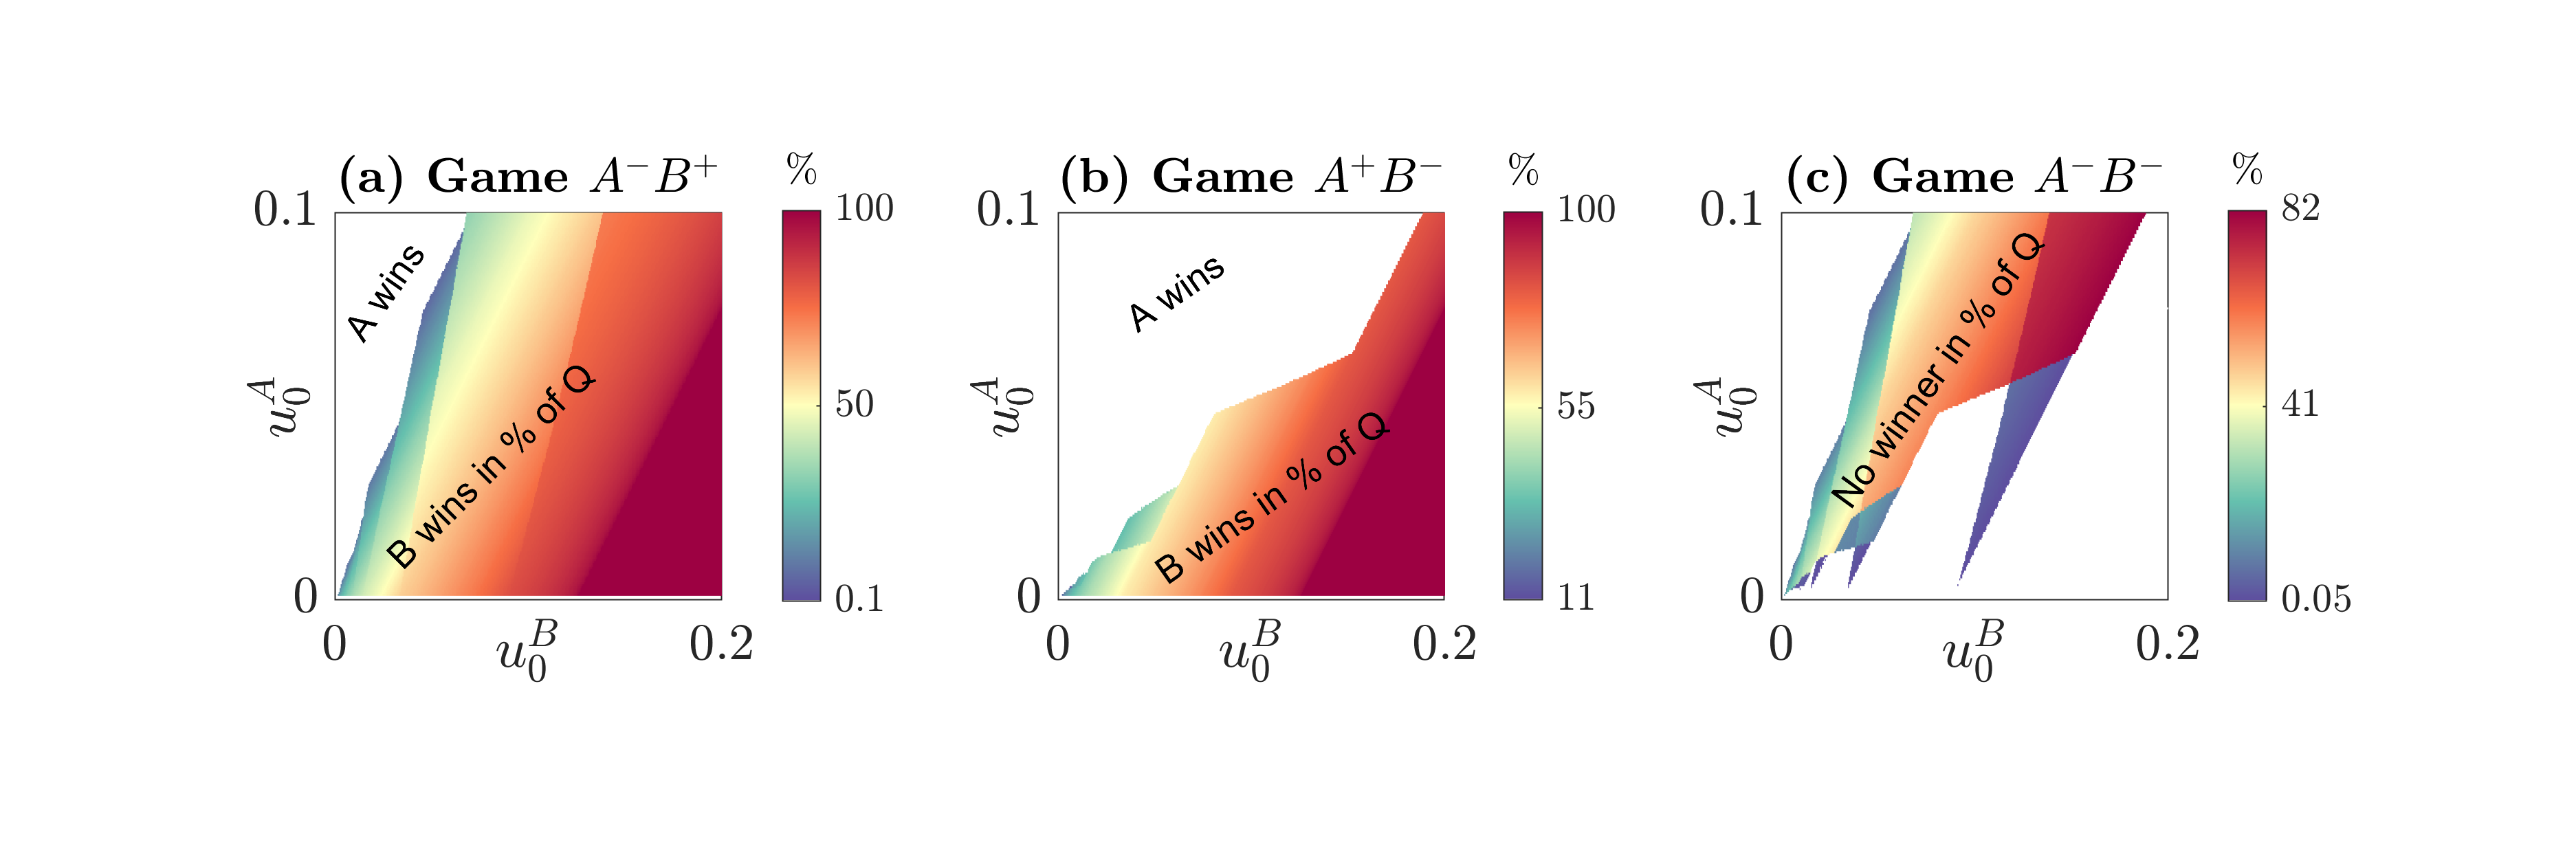
\includegraphics[trim={3.1cm 0cm 0cm 0cm}, clip,width=1.12\textwidth  ]{Images/P5/fraccion.png}
    \caption{The first two panels show the percentage of the region that occupies the winning set of player $B$ respect region $Q$ whether they are informed (+) or ignorant (-). The color is white when the percentage is zero. The last panel represents the percentage of initial conditions that do not assure a winner when both players are ignorant. All figures show similar details at different scales, suggesting self similarity in the system dynamics.}
    \label{fig:fraccion}
\end{figure}













The results of these games are heavily influenced by the range of control available to each player. Figure~\ref{fig:franjas} offers a detailed exploration of potential game scenarios within the parameter space $(u_0^B, u_0^A) \in [0,0.2] \times [0,0.1]$. It distinguishes between three types of games:  $A$ ignorant vs $B$ informed, $A$ informed vs $B$ ignorant, and both players ignorant.

In these diagrams, certain regions represent scenarios where one player is guaranteed to win regardless of the starting conditions, while other regions show outcomes that depend on the initial setup. In particular, when both players lack information (Fig.~\ref{fig:franjas}(c)), there are regions labeled as $NW$ (no winner) that represent cases where the outcome is indeterminate for certain starting conditions.

The lower panels (Figs.~\ref{fig:franjas}(d-f)) provide concrete examples of winning sets for five different parameter combinations, referred to as games $P1$ through $P5$. These examples illustrate how winning sets change as the parameters vary across the identified regions of the parameter space.

Figure~\ref{fig:fraccion} further analyzes these findings by showing the proportion of region $Q$ occupied by each player's winning set. Notably, Fig.~\ref{fig:fraccion}(c) highlights the percentage of initial conditions where neither player can secure a guaranteed win when both are unaware. The color gradients in this figure depict a gradual shift in game outcomes as control bounds change.

These findings emphasize how the relative strength of the players' control bounds shapes not only who emerges victorious but also whether a definitive victory is possible. When the control bounds are closely matched, the results often depend on initial conditions or remain uncertain.


\subsection{Boundary games}

\begin{figure}
    \centering
    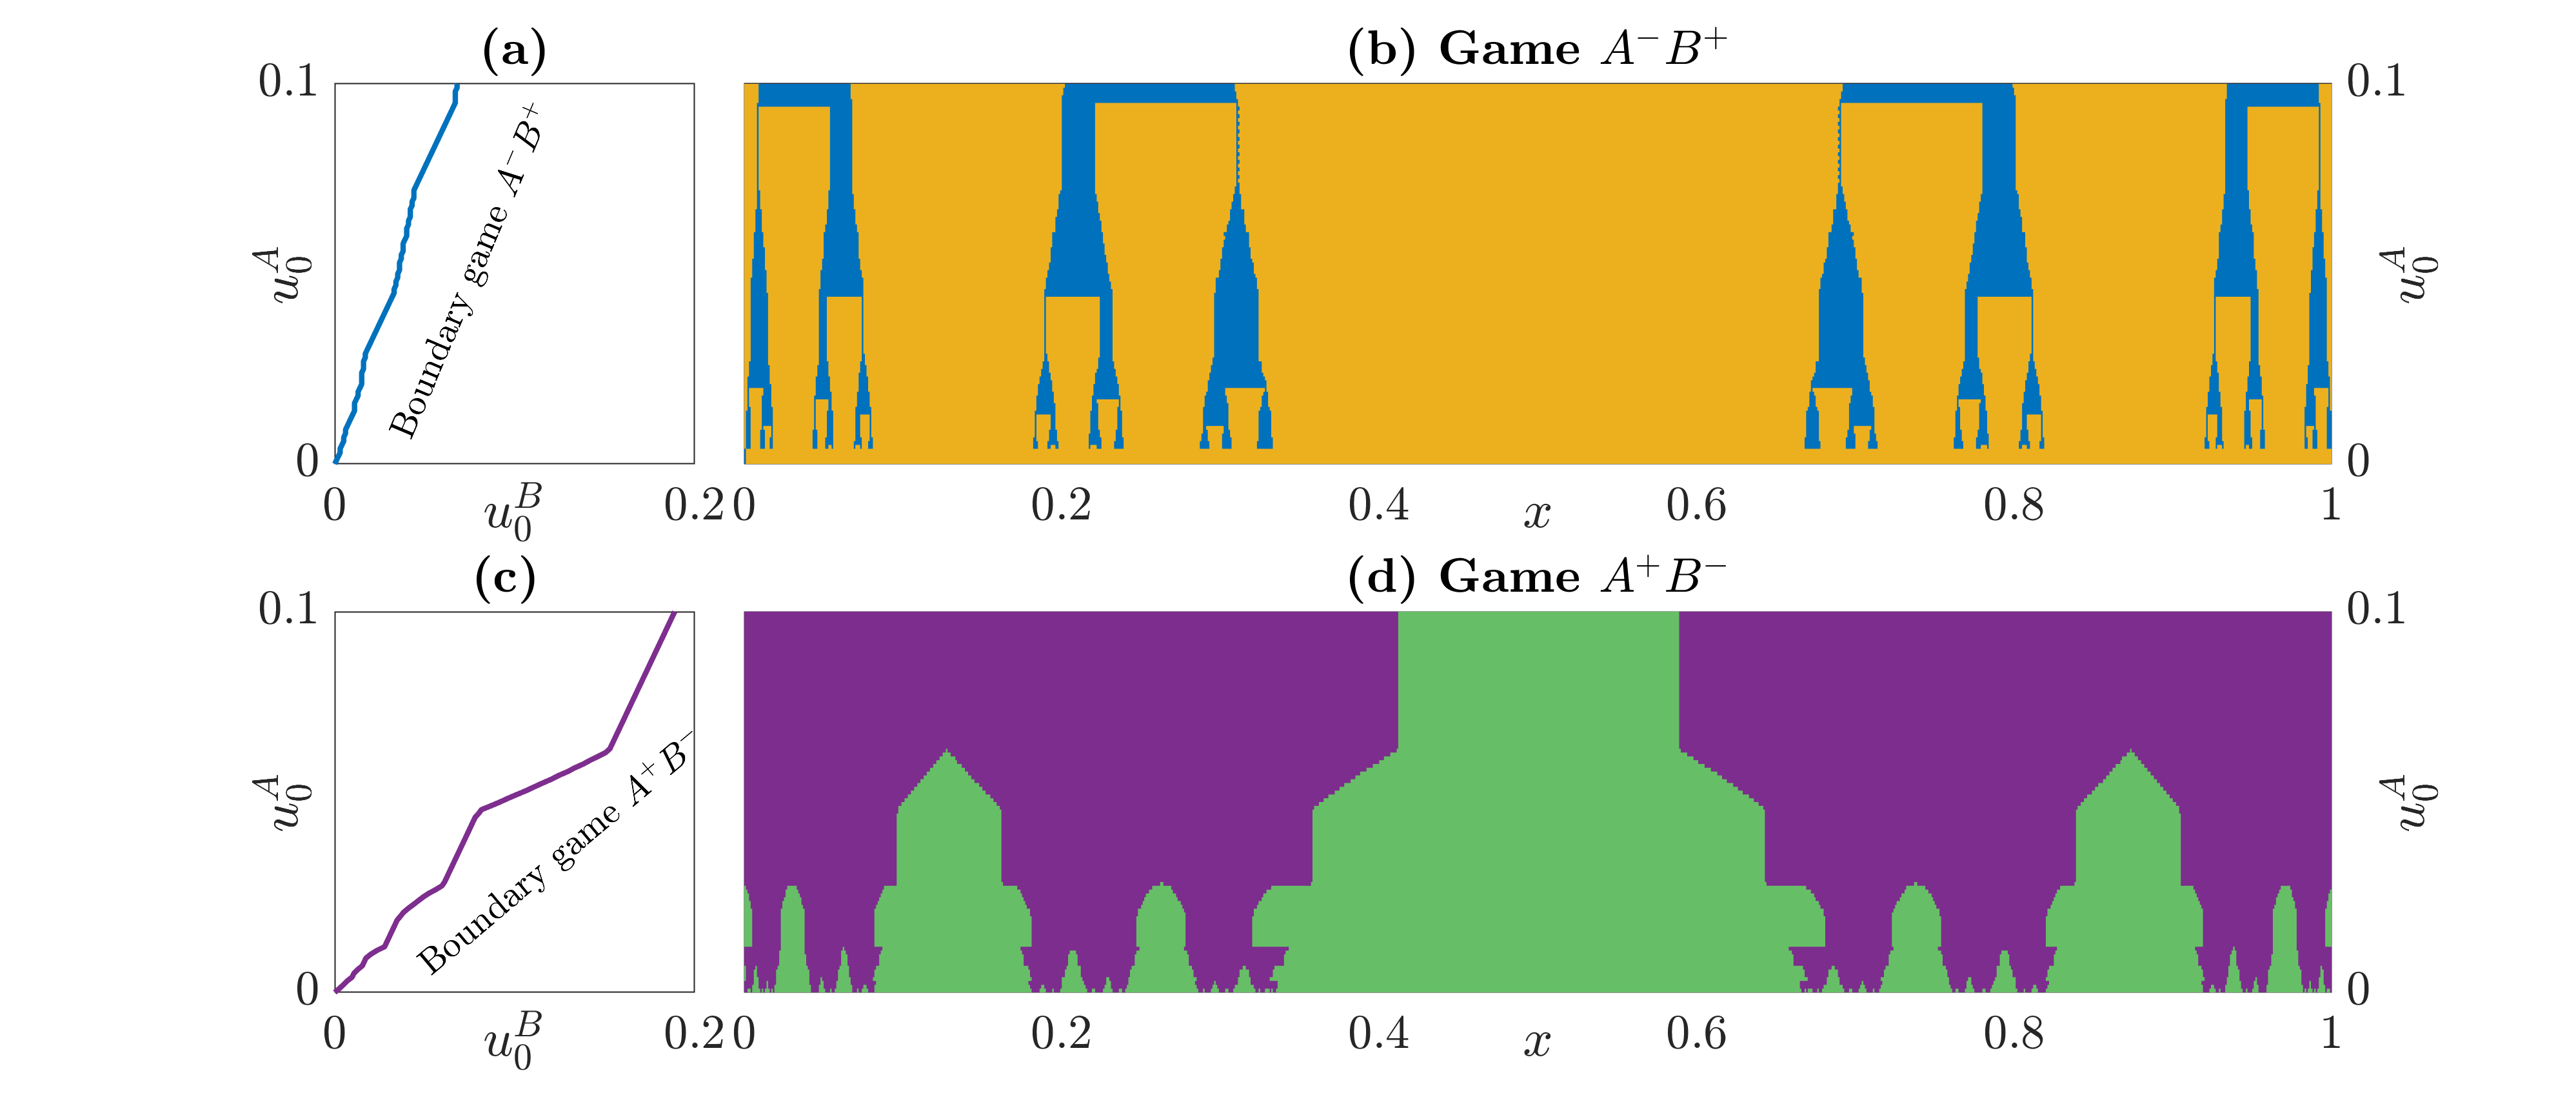
\includegraphics[trim={3.3cm 0cm 0cm 0cm}, clip,width=1.06\textwidth ]{Images/P5/bifurcation.png}
    \caption{Panels (a) and (c) show the game boundary for which there is a shift between player $A$ winning the game at all initial conditions (left of the line) and there is a mixed victory among different initial conditions (right of the line). This lines are the boundaries of panels (a) and (b) from the previous figure. Panels (b) and (d) show the winning sets within the control bounds along the game boundary. In colors yellow and blue the points in the $A$ ignorant and $B$ informed winning sets respectively and in green and purple, $A$ informed and $B$ ignorant. In panel (b) we can clearly see increasing and almost self-similar details when the scales decreases.}
    \label{fig:bifurcation}
\end{figure}







The dynamics of the game inherently favor player $A$, whose objective is to exit region $Q$, a process that occurs naturally due to the transient nature of the system. However, this does not mean player $B$ is without hope. With sufficient control, player $B$ can still achieve their goal. The boundary games depicted in Fig.~\ref{fig:bifurcation} examine the critical limits of control at which player $B$’s victories begin to emerge. This boundary, illustrated in Figs.~\ref{fig:bifurcation}(a) and~\ref{fig:bifurcation}(c) within the $(u_0^B, u_0^A)$ parameter space, marks a pivotal transition: slightly increasing $u_0^A$ or reducing $u_0^B$ results in a scenario where player $B$ cannot win under any conditions. Conversely, crossing this boundary creates initial conditions where $B$’s victory becomes possible.

The structure of these boundaries is particularly noteworthy, as shown in Figs.~\ref{fig:bifurcation}(b) and~\ref{fig:bifurcation}(d), which present the winning sets along these transitions for two distinct game types. In the case of $A$ ignorant vs $B$ informed (Fig.~\ref{fig:bifurcation}(b)), we see a highly intricate pattern of $B$’s victories, represented as blue regions within $A$’s domain. These patterns exhibit increasing detail at finer scales, hinting at a self-similar structure. By contrast, in the scenario where $A$ is informed and $B$ ignorant (Fig.~\ref{fig:bifurcation}(d)), the arrangement takes on a different form, with $B$’s victory regions (purple) interspersed with $A$’s (green) in a complex but distinct alternating pattern.






The dynamics of the game inherently favor player $A$, whose objective is to exit region $Q$, a process that occurs naturally due to the transient nature of the system. However, this does not mean player $B$ is without hope. With sufficient control, at some cases even with control lower than that of player $A$, player $B$ can still achieve their goal. The boundary games depicted in Fig.~\ref{fig:bifurcation} examine the critical limits of control at which player $B$’s victories begin to emerge. This boundary, illustrated in Figs.~\ref{fig:bifurcation}(a) and~\ref{fig:bifurcation}(c) within the $(u_0^B, u_0^A)$ parameter space, marks a pivotal transition, crossing this boundary creates initial conditions where $B$’s victory becomes possible. 




The structures shown in Figs.~\ref{fig:bifurcation}(b) and~\ref{fig:bifurcation}(d), which present the winning sets along these transitions for two distinct game types, are of great interest. In the case of $A$ ignorant vs $B$ informed (Fig.~\ref{fig:bifurcation}(b)), we see a highly intricate pattern of $B$’s victories, represented as blue regions within player $A$’s domain, depicted in yellow. These patterns exhibit increasing detail at finer scales, hinting at a self-similar structure. By contrast, in the scenario where player $A$ is informed and player $B$ is ignorant (Fig.~\ref{fig:bifurcation}(d)), the arrangement takes on a different form, with player $B$’s victory regions (purple) alternating with player $A$’s (green) in a complex but distinct pattern.






\subsection{Is it worth being informed?}


\begin{figure}
    \centering
    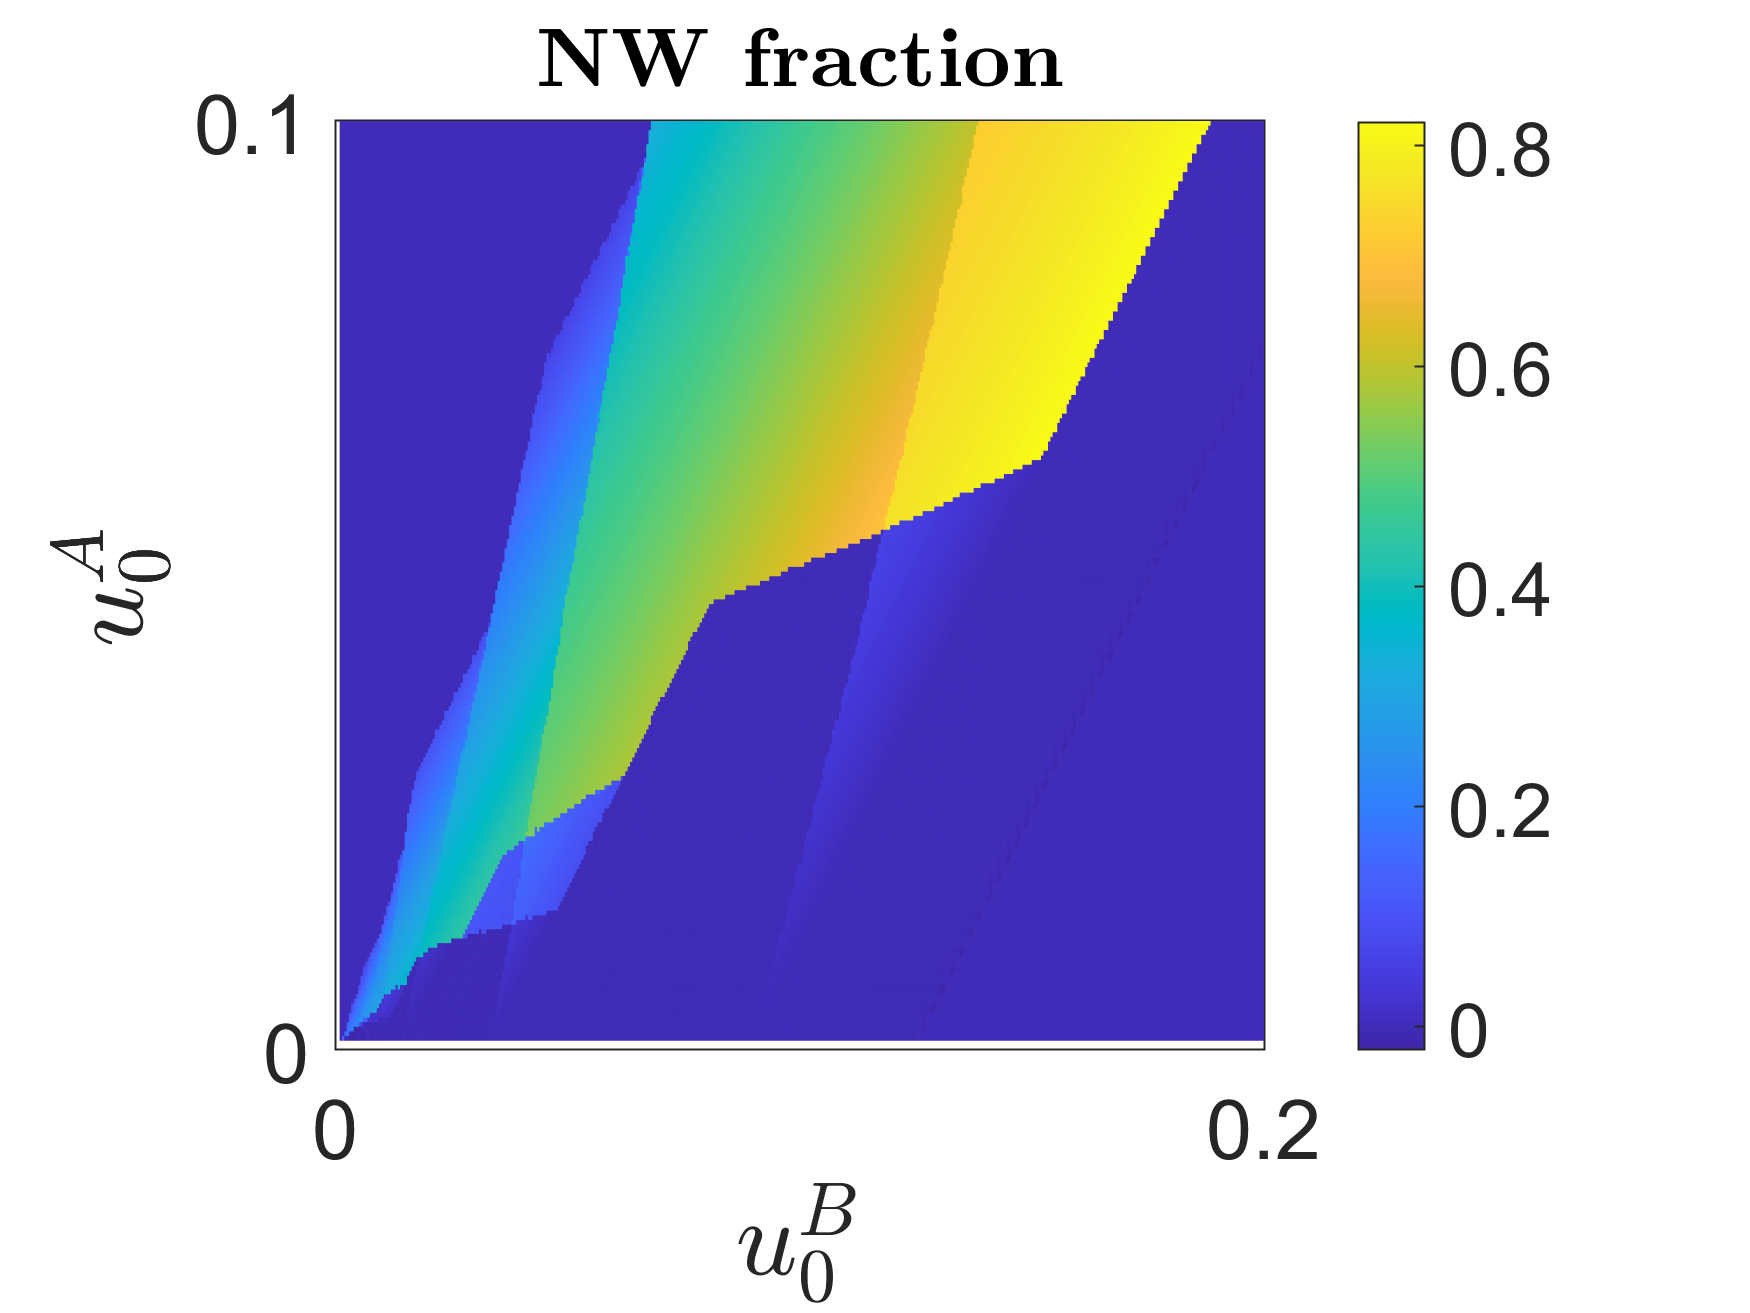
\includegraphics[trim={0cm 0cm 0cm 0cm}, clip,width=0.5\textwidth ]{Images/P5/diferencia.png}
    \caption{The color on the heatmap represents the difference between the informed and ignorant sets fraction. The no winning fraction ($NW$) satisfies the relation $NW = A^{+} - A^{-} = B^{+} - B^{-}$, that is, the difference is the same for both players. Therefore they will fight for being the one informed at the same parameter regions. However for many points the difference is $0$, so being informed or being ignorant results in the same winning set.}
    \label{fig:diferencia}
\end{figure}


The advantage of playing second in this game is evident because they have the knowledge of the opponent's actions, as this allows them to counteract any move the rival makes. Consequently, the ignorant sets are strictly contained within the informed sets. Interestingly, when plotting the difference between the proportions of each player's informed and ignorant sets (Fig.~\ref{fig:diferencia}), we observe a large region where this difference is zero. Notably, this region corresponds to the same area in Fig.~\ref{fig:fraccion} where no player can guarantee victory. This relationship is clearly demonstrated by the following equations:
\begin{equation}
   \left. \begin{array}{lll}
        &A^{+} + B^{-} = 1 \\
        &A^{-} + B^{+} = 1 \\
        &A^{-} + B^{-} + NW = 1
    \end{array}
    \right\} \Rightarrow NW = A^{+} - A^{-} = B^{+} - B^{-}.
\end{equation}
Here, $P^{+}$ represents the proportion of region $Q$ occupied by the winning set of the informed player $P$, while $P^{-}$ denotes the same proportion for the ignorant player. The term $NW$ (no winning) corresponds to the proportion of blank space when both players are ignorant.



If players could compete for the right to act as the informed player, it is reasonable to assume that there would be a cost associated with gaining this advantage. In such a scenario, it may not always be worthwhile to incur the cost of being informed, because in a significant portion of cases, the outcome remain unchanged. However, if minimizing the average control effort is a priority, being informed offers a substantial advantage in nearly all situations. We have checked that the minimal control required to obtain the same results is lower for informed players.



\section{Conclusions}

We proposed a novel two-player game of survival in a transient chaotic region. In the game, two players are confronted against each other to control the trajectory of a chaotic dynamical system. The players had opposing goals, each one aiming to get the trajectory to different regions. Through the partial control method we got the set of initial points that guaranteed the victory for each player. Through partial control algorithms we were able to construct winning sets that provided the initial conditions where each player had victory assured. Then, the controlled trajectories are not unique, but at each iteration of the game, the system can be controlled to a range of possible points within the winning sets, giving more flexibility to the controllers.

We applied the game to the logistic map. Here one player aims to stay at the transient chaotic region and the rival wants to drive the trajectory out of there. This system unveils an interesting aspect about the complexity of the dynamical system. Because even when the dynamical system plays against the conservative player and their opponent has greater control capabilities, the player can thrive and achieve their objective.

We also found that the information each player has plays a substantial role in the game. The player that plays first, and therefore knows the action of the rival, will undoubtedly be at an advantage. Therefore, this knowledge was crucial to victory at some cases, but at some other cases, surprisingly, the information was of little use to the informed player.

Finally another interesting result is that when no player knows the action of their rival, regions appear where victory is uncertain. The game is unresolved there and the outcome will depend on the sequence of actions of the players.



\begin{thebibliography}{04}





\bibitem{Yorke}
J. Aguirre, F. d’Ovidio, and M. A. F. Sanjuán,
Controlling chaotic transients: Yorke’s game of survival.
Phys. Rev. E 69:016203
(2004)
\url{https://doi.org/10.1103/PhysRevE.69.016203}



\bibitem{DynamicsPartialControl}
Juan Sabuco, Miguel A. F. Sanjuan, and James A. Yorke
Dynamics of partial control
Chaos 22:047507
(2012)
\url{https://doi.org/10.1063/1.4754874}


\bibitem{PartialControlBeyond}
R.~Cape{\'a}ns, J.~Sabuco, and M.~A.~F. Sanju{\'a}n, 
Beyond partial control: controlling chaotic transients
with the safety function.
Nonlinear Dyn. 107:2903–2910
(2022)
\url{https://doi.org/10.1007/s11071-021-07071-1}

\bibitem{PartialControlFunctions}
R.~Cape{\'a}ns, J.~Sabuco, and M.~A.~F. Sanju{\'a}n, 
A new approach of the partial control method in chaotic systems.
Nonlinear Dyn. 98:873--887
(2019)
\url{https://doi.org/10.1007/s11071-019-05215-y}

\bibitem{PartialControlEscape}
G. Alfaro, R.~Cape{\'a}ns, and M.~A.~F. Sanju{\'a}n, 
Forcing the escape: Partial control of escaping orbits from a
transient chaotic region.
Nonlinear Dyn. 104:1603–1612
(2021) 
\url{https://doi.org/10.1007/s11071-021-06331-4}





\bibitem{Social}
P. Kollock,
Social dilemmas: the anatomy of cooperation.
Annu. Rev. Sociol. \textbf{24}, 183-214
(1998)
\url{https://doi.org/10.1146/annurev.soc.24.1.183}

\bibitem{EconomyGames}
Y. Xiao, Y. Peng, Q. Lu, and X. Wua,
Chaotic dynamics in nonlinear duopoly Stackelberg game
with heterogeneous players.
Physica A \textbf{492}, 1980--1987
(2018)
\url{https://doi.org/10.1016/j.physa.2017.11.112}

\bibitem{GamesComplex}
W. Hu, G. Zang, H. Tian. and Z. Wang,
Chaotic dynamics in asymmetric rock-paper-scissors games.
IEEE Access \textbf{7}, 175614--175621
(2019)
\url{https://doi.org/10.1109/ACCESS.2019.2956816}

\bibitem{AkiyamaKaneko1}
E. Akiyamaa and K. Kaneko,
Dynamical systems game theory and dynamics of games,
Physica D \textbf{147}, 221--258
(2000)
\url{}

\bibitem{AkiyamaKaneko2}
E. Akiyamaa and K. Kaneko,
Dynamical systems game theory II
A new approach to the problem of the social dilemma
Physica D \textbf{167}, 36--71
(2002)
\url{https://doi.org/10.1016/S0167-2789(00)00157-3}

\bibitem{GamesControl}
J. R. Marden and J. S. Shamma,
Game Theory and Control.
Annu. Rev. Control. Robotics Auton. Syst. \textbf{1}, 105--134
(2018)
\url{https://doi.org/10.1146/annurev-control-060117-105102}

\bibitem{PartialControlGame}
G. Alfaro, R. Capeáns, M. A. F. Sanjuán,
Two-player Yorke's game of survival in chaotic transients,
(2025)
\url{https://doi.org/10.48550/arXiv.2501.12188}


\end{thebibliography}